\documentclass{article}
\usepackage[utf8]{inputenc}
\usepackage{polski}
\usepackage{graphicx}
\usepackage[margin= 3cm]{geometry}


\title{Wskaźnik MACD}
\author{Piotr Pesta}
\date{Marzec 2022}
\setlength{\parindent}{20pt}
\graphicspath{{./Graphs/}}

\begin{document}
\maketitle

\section{Wstęp}
    Wskaźnik MACD składa się z dwóch linii:
    \begin{itemize}
        \item MACD
        \item Signal (tzw. sygnał)
    \end{itemize}

    Linia \textbf{MACD} tworzona jest na podstawie róznicy dwóch średniej krótkookresowej i długookresowej.
    W przypadku tego projektu są to średnie kroczące z 12 i 26 okresów.

    Linia \textbf{Signal} powstaje natomiast na podstawie średniej kroczącej z wartości wskaźnika MACD z 9 okresów.

    Momenty kupna i sprzedaży wyznaczają momenty przecięcia krzywych MACD oraz Signal. Gdy MACD przecina
    Signal od dołu, jest to sygnał do zakupu akcji i początek trendu wzrostowego. Natomiast w przypadku gdy MACD przecina Signal od góry
    oznacza to moment sprzedaży i zapowiedź odwrócenia trendu.

\section{Przykład działania}
    Lorem Ipsum is simply dummy text of the printing and typesetting industry. Lorem Ipsum has been the industry's standard dummy text ever since the 1500s, when an unknown printer took a galley of type and scrambled it to make a type specimen book. It has survived not only five centuries, but also the leap into electronic typesetting, remaining essentially unchanged. It was popularised in the 1960s with the release of Letraset sheets containing Lorem Ipsum passages, and more recently with desktop publishing software like Aldus PageMaker including versions of Lorem Ipsum.


   \noindent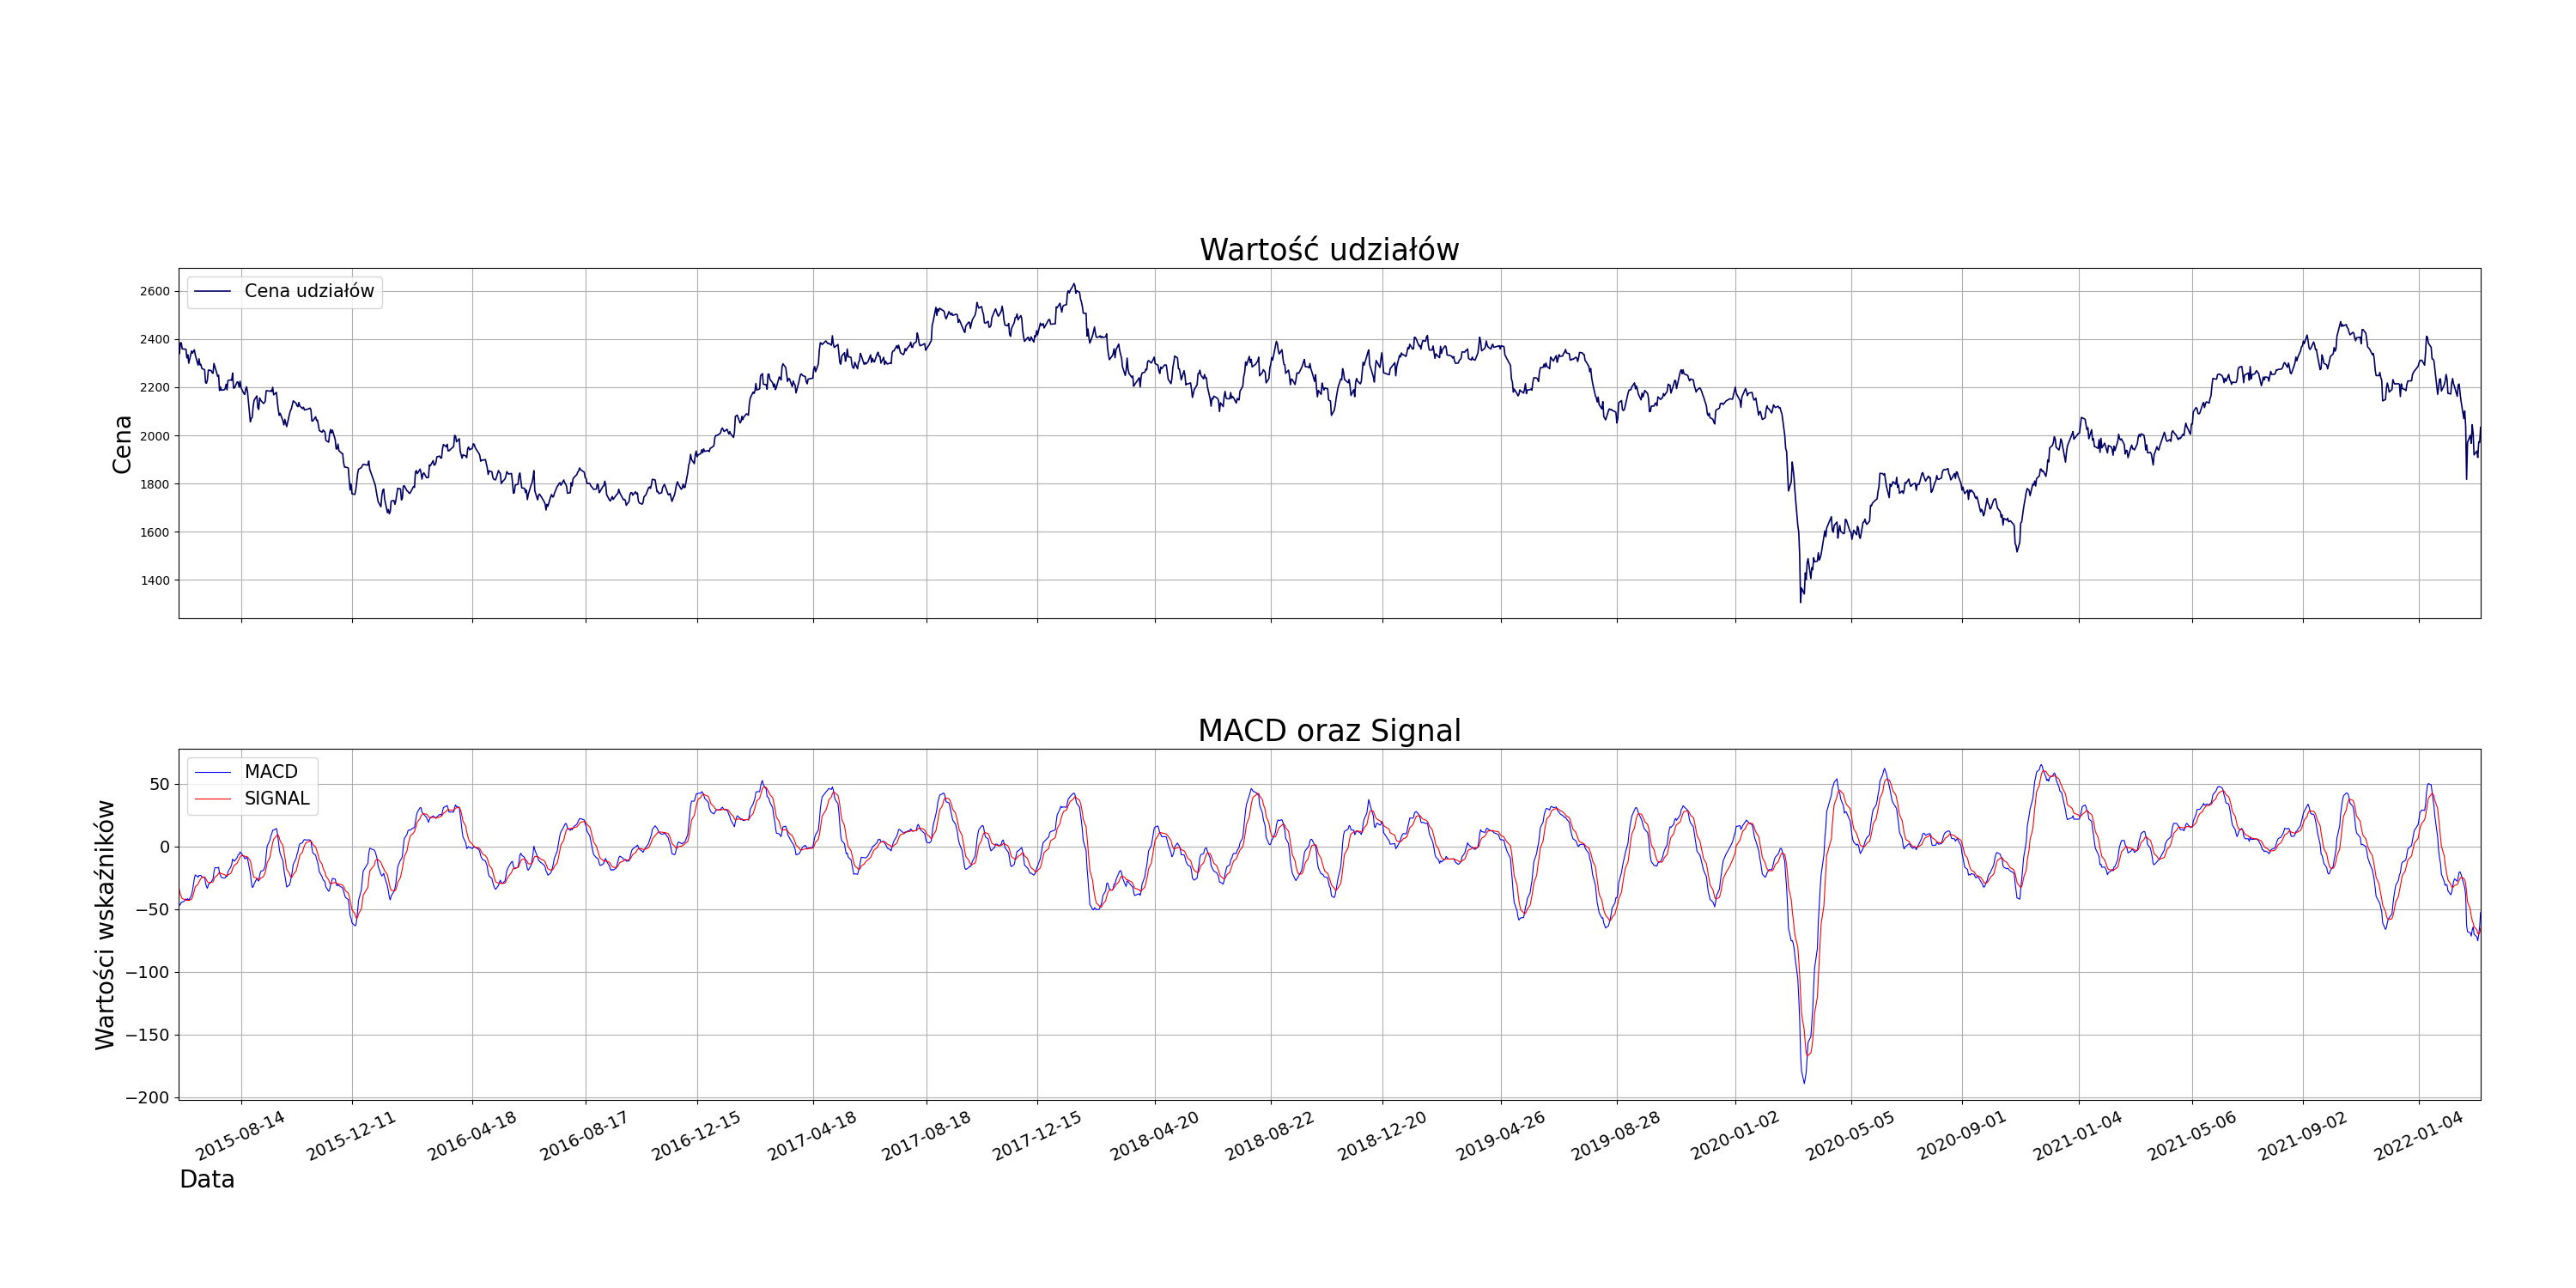
\includegraphics[width=\textwidth]{WIG20}
    \centering

\section{Analiza przydatności MACD do inwestowania}

    Tutaj analiza algorytmu do inwestowania

\end{document}